%%%%%%%%%%%%%%%%%%%%%%%%%%%%%%%%%%%%%%%%%%%%%%%%%%%%%%%%%%
%%
%% MARK: Title
%%
%%%%%%%%%%%%%%%%%%%%%%%%%%%%%%%%%%%%%%%%%%%%%%%%%%%%%%%%%%

\chapter*{\S B24. The Diffeomorphisms of the Square}
\setcounter{footnote}{0}

%%%%%%%%%%%%%%%%%%%%%%%%%%%%%%%%%%%%%%%%%%%%%%%%%%%%%%%%%%
%%
%% MARK: Abstract
%%
%%%%%%%%%%%%%%%%%%%%%%%%%%%%%%%%%%%%%%%%%%%%%%%%%%%%%%%%%%

\begin{abstract}
  In this note we shall see how diffeology,
  understood as the geometry of the group of diffeomorphisms in the sense of Felix Klein,
  fulfills its duty concerning the full square $\text{Sq} = [0,1]^2 \subset \RR^2$.
\end{abstract}

%%%%%%%%%%%%%%%%%%%%%%%%%%%%%%%%%%%%%%%%%%%%%%%%%%%%%%%%%%
%%
%% MARK: Content
%%
%%%%%%%%%%%%%%%%%%%%%%%%%%%%%%%%%%%%%%%%%%%%%%%%%%%%%%%%%%

\vspace{-1em}
According to Klein's program \cite{Kle72},
a geometry is often understood as the action of a group (called the {\em principal group}) on some space.
As an example, Euclidean geometry is the action of the Euclidean group on a Euclidean space,
affine geometry,
the action of the affine group, etc.
Without committing to a dogmatic interpretation of this principle,
the example of the closed square discussed here,
in the diffeology framework,
illustrates how the action of the diffeomorphism group captures fine geometric distinctions
---~such as corners versus edges versus interior~---
that pure topology cannot see.

\begin{Article}{Klein decomposition.}{}
  Let $\text{Sq} = [0,1]^2 \subset \RR^2$ be equipped with the subset diffeology.
  The decomposition of the square under the group of diffeomorphisms yields the expected three orbits:
  
  \begin{enumerate}
    \item The $4$ corners: $\text{NO}=(0,1)$,
    $\text{NE}=(1,1)$,
    $\text{SO}=(0,0)$ and $\text{SE}=(1,0)$.
    \item The $4$ edges: $\text{B} = ]0,1[ \times \{0\}$,
    $\text{T} = ]0,1[ \times \{1\}$,
    $\text{L} = \{0\} \times ]0,1[$ and $\text{R} = \{1\} \times ]0,1[$.
    \item The interior $\mathring{\text{Sq}} = ]0,1[^2$.
  \end{enumerate}
\end{Article}

\Note{1.} The quotient diffeology on
$$\text{Sq}/\Diff(\text{Sq}) = \{\text{Corners},\text{Edges},\text{Interior}\}$$
is of course not the discrete diffeology;
it captures the combinatorial structure of the orbits.

\Note{2.} Under homeomorphisms there are only $2$ orbits,
the boundary and the interior.
In our case,
the differential structure is obviously indispensable.

\begin{proof}
  (1) Let us show that $\text{Sq}$ is embedded in $\RR^2$.
  That is,
  the D-topology of the induction $\text{Sq} \subset \RR^2$ coincides with the induced topology of $\RR^2$.
  For any subset $\U \subset \text{Sq}$ open in the induced topology,
  there exists an open $\cO \subset \RR^2$ such that $\U = \cO \cap \text{Sq}$.
  For all plots $P$ in $\text{Sq}$,
  $P^{-1}(\U) = P^{-1}(\cO)$ is open,
  because plots are continuous.
  On the other hand,
  let $\U \subset \text{Sq}$ be D-open.
  Then $s^{-1}(\U)$ is open,
  where $s \colon \RR^2 \to \text{Sq}$ is the map $s(x_1,x_2) = (x_1^2, x_2^2)$.
  Moreover, $s^{-1}(\U) \cap \text{Sq}$ is open in the induced topology of $\RR^2$.
  Now,
  the map $s$ restricted to $\text{Sq}$ is a homeomorphism.
  Hence,
  since $\U = s(s^{-1}(\U) \cap \text{Sq})$,
  $\U$ is open in the induced topology of $\RR^2$.
  Therefore the D-topology of the induction coincides with the induced topology.
  
  (2) Now,
  let us show that a diffeomorphism of $\text{Sq}$ cannot send a point of the boundary into the interior.
  Let $f \colon \text{Sq} \to \text{Sq}$ be a diffeomorphism for the subset diffeology.
  Hence $f$ is a homeomorphism for the D-topology.
  Assume that $f$ maps $x \in \text{L}$ to $f(x) \in \mathring{\text{Sq}}$.
  Obviously $f$ induces a homeomorphism
  $\tilde{f} \colon \text{Sq} \setminus \{x\} \to \text{Sq} \setminus \{f(x)\}$.
  Since $x \in \text{L}$,
  we have that $\text{Sq} \setminus \{x\}$ is convex,
  therefore homotopy equivalent to a point.
  On the other hand,
  we can construct a homotopy equivalence
  $\text{Sq} \setminus \{f(x)\} \simeq \partial \text{Sq} \simeq \Sph^1$.
  Thus,
  we would obtain $\{\text{point}\} \simeq \Sph^1$,
  which is a contradiction.
  
  (3) A diffeomorphism of the square must send corners to corners.
  Let $f$ be a diffeomorphism of $\text{Sq}$,
  such that $f \restriction \text{L}$ takes values in $\text{L} \cup \text{SO} \cup \text{B}$,
  and the restriction of $f$ to $\text{L}$ is defined as follows:
  $$
    f(t e_2) =
    \begin{cases}
      \phi(t) e_1, & \text{if } 0 < t < \frac{1}{2} \\
      \text{SO},   & \text{if } t = \frac{1}{2} \\
      \psi(t) e_2, & \text{if } \frac{1}{2} < t < 1
    \end{cases}
  $$
  where $e_1$ and $e_2$ are the vectors of the canonical basis of $\RR^2$.
  
  Thus,
  for all $p > 0$,
  $$
    \lim_{t \to \frac{1}{2}^-} f^{(p)}(t e_2) = \phi^{(p)}(t) e_1
    \quad \text{and} \quad
    \lim_{t \to \frac{1}{2}^+} f^{(p)}(t e_2) = \psi^{(p)}(t) e_2.
  $$
  Hence by continuity,
  for all $p > 0$,
  $\phi^{(p)}\!\left(\frac{1}{2}\right) = \psi^{(p)}\!\left(\frac{1}{2}\right)$.
  
  Therefore,
  $f$ is flat at $\frac{1}{2}$.
  The restriction of $f^{-1}$ to $\text{L} \cup \text{SO}$ is a local diffeomorphism of half-space with the subset diffeology.
  By \cite[\textsection\,4.14]{PIZ13} (a consequence of \cite{Whi43}),
  there exists $F \in \Cinfty(]-\epsilon, 1[, \RR)$ such that
  $f^{-1} \restriction \text{L} \cup \text{SO} = F \restriction \text{L} \cup \text{SO}$.
  We have $f^{-1}(f(t)) = t$,
  for all $t > \frac{1}{2}$.
  Thus,
  $(f^{-1})'(f(t)) f'(t) = 1$.
  But
  $(f^{-1})'(f(t)) f'(t) = \lim_{t \to \frac{1}{2}} F'(f(t)) f'(t) = 0$,
  which is a contradiction.
  Therefore the $4$ corners of $\text{Sq}$ form an orbit of $\Diff(\text{Sq})$.
\end{proof}

\medskip
\begin{figure}[h]
  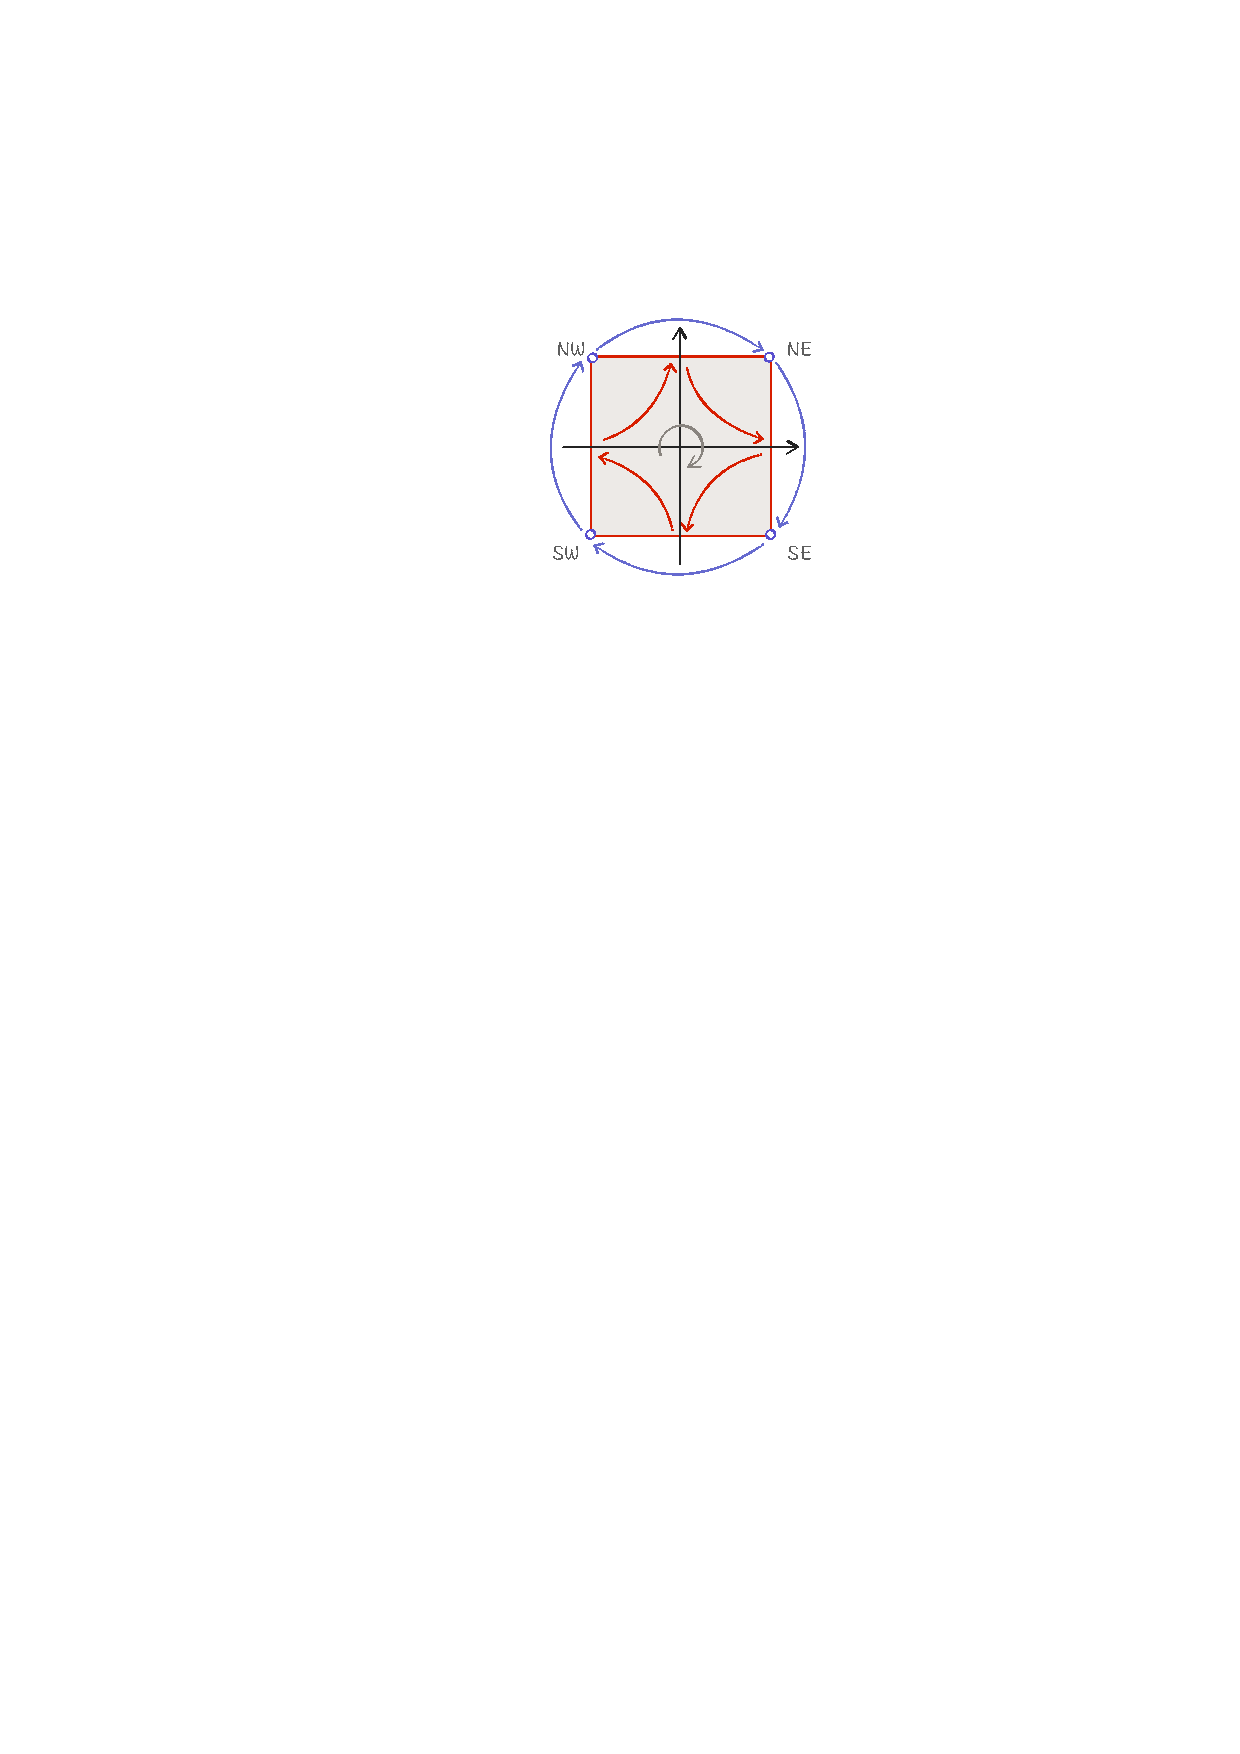
\includegraphics[width=.75\textwidth]{Figures/Square.pdf}
  %\vspace{-.25\baselineskip}
  \caption{The diffeomorphisms of the square.}
  \label{The diffeomorphisms of the square}
\end{figure}
